\documentclass[11pt,a4paper]{article}
\usepackage[onecolumn,papersize=a4paper,margin=2.2cm,parskip]{kr-zh}

\usepackage{listings}
\usepackage{tabularx}
\usepackage{longtable}
\usepackage{subcaption}
\usepackage{xcolor}
\usepackage{graphicx}

\usepackage{float}
\usepackage{booktabs}
\usepackage{multirow}
\usepackage{graphicx}
\usepackage{caption}

\usepackage[backend=biber,style=numeric,natbib=true]{biblatex}
\addbibresource{references.bib}

\title{FGLP:Fine-Grained Learning Path Recommendation Based on Hierarchical Two-Stage Decision-Making}

% Single author syntax
\author{%
    Zijie Liao
    \affiliations
    Guangdong Institute of Smart Education, Jinan University, Guangzhou, China
    \emails
    fenglin@stu2025.jnu.edu.cn
}


\begin{document}
\maketitle

\begin{abstract}
 学习路径推荐旨在根据学习者的知识状态与学习目标，动态生成个性化的学习项目序列，是在线教育中实现自适应学习的重要任务。现有方法通常借助知识追踪或强化学习建模学习过程，但仍存在三方面不足：一是学习收益评价多依赖掌握阈值下的二元判断，难以刻画阈值两侧的细粒度状态变化；二是分层推荐方法往往将知识点规划与习题选择割裂建模，导致高层策略难以及时感知习题交互带来的状态反馈；三是多数方法缺少对剩余学习预算的显式建模，难以区分不同学习进程下的推荐需求。为解决上述问题，本文提出一种基于分层两阶段决策的细粒度学习路径推荐框架 FGLP。该框架通过统一学生状态估计模块同时建模知识点级与习题级掌握状态，并采用“一步一知识点一习题”的决策粒度实现知识点推荐层与习题推荐层之间的即时反馈。在知识点推荐层，本文引入目标推进与目标巩固两阶段机制，并结合二元学习收益、连续学习收益与预算感知奖励，以提升有限预算下的目标达成效率和状态保持能力；在习题推荐层，本文采用状态感知的两塔匹配与 bandit 式局部决策，并利用一步前瞻收益构造监督信号，从而选择更符合当前学习状态的练习题。我们在Junyi、Assist09 和 Assist17 三个公开数据集中进行了大量的实验,结果证明了我们方法的能够显著提升学生的学习收益.   
\end{abstract}

\section{Introduction}
随着在线教育平台的快速发展，学习者可以自由访问海量学习资源\cite{korableva2019studying,zhang2019hierarchical}。然而，资源丰富性也带来了信息过载问题：缺乏引导的学习者往往难以在庞杂材料中确定合适的学习顺序，导致学习路径碎片化和学习效率下降。学习路径推荐（Learning Path Recommendation, LPR）旨在根据学习者的知识状态与学习目标，动态生成个性化的学习项目序列，从而引导学习者更高效地完成目标导向学习\cite{nabizadeh2020learning,guan2025explainable,liu2019exploiting}。

早期学习路径推荐方法主要依赖知识结构、启发式搜索或传统序列推荐模型\cite{yu2007ontology,nabizadeh2020adaptive,zhou2018personalized,zhu2018multi}。近年来，知识追踪（Knowledge Tracing, KT）技术\cite{piech2015deep,shen2022assessing,liu2025deep}的发展使系统能够动态估计学生知识状态\cite{kubotani2021rltutor,}，强化学习（Reinforcement Learning, RL）也被进一步用于建模长期学习收益下的序列决策过程\cite{liu2019exploiting,li2023graph,chen2023set,cheng2026graphrag}。尽管这些方法提升了路径推荐的动态性，但在目标导向场景中仍存在若干关键不足。如图~\ref{fig:method-comparison} 所示，现有方法的局限主要体现在奖励设计与决策粒度两个方面：一方面，终局奖励只能在学习路径结束后提供反馈\cite{liu2019exploiting}，导致策略学习信号稀疏；以密集奖励为代表的改进方法虽然能够提供步级反馈\cite{peng2026uno}，但通常仍依赖掌握阈值下的二元判断，难以刻画阈值以下的渐进改善以及达标后的进一步提升.例如,当掌握阈值为0.6时,将掌握水平从0.2提升到0.5会被视为“没有提升”,而从0.6提升到0.9也难以被体现为进一步的进步。另一方面，现有将习题引入学习路径推荐的方法通常将知识点规划与具体习题选择拆分为两个相对独立的任务\cite{zhang2024item,cheng2026graphrag,li2023graph}，并依赖规则预算分配进行衔接，使高层策略难以及时感知习题交互带来的细粒度状态变化，也难以自适应判断某个知识点需要多少次练习。此外，目前已有的方法都缺少对剩余学习预算的显式建模，因而难以区分相同知识状态但处于不同学习进程的学生需求,从而影响到学生的学习效率。

\begin{figure} % 位置参数，见下文解释
    \centering % 图片居中
    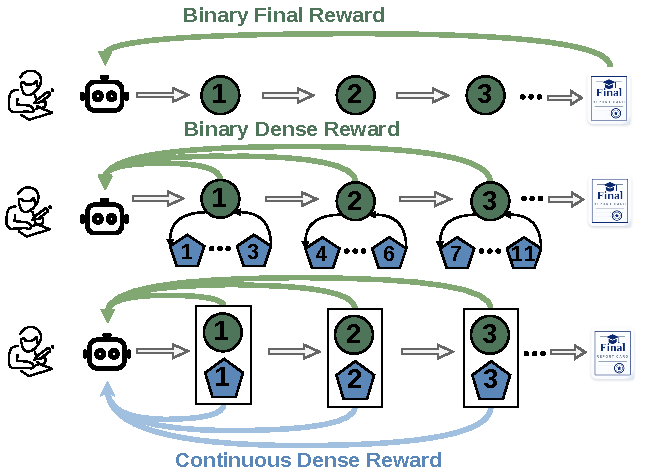
\includegraphics[width=\columnwidth]{illustration_new.pdf} % 插入图片并设置宽度
    \caption{Motivating comparison of reward design and decision granularity for fine-grained learning path recommendation.}
    \label{fig:method-comparison} % 用于交叉引用的标签
\end{figure}

为此，本文提出基于分层两阶段决策的细粒度学习路径推荐框架。该框架由统一学生状态估计模块、知识点推荐层与习题推荐层组成：状态估计模块同时输出知识点级与习题级掌握状态；决策过程采用"一步一知识点一习题"的粒度，知识点层选择知识点、习题层选择习题，并在交互后即时更新状态，使知识点层能够感知习题带来的细粒度变化。知识点层引入双阶段目标导向机制，将学习过程划分为目标推进与目标巩固，并结合连续学习收益和预算嵌入刻画细粒度进展与剩余学习进程；习题层采用状态感知的两塔匹配与bandit式局部决策，在当前知识点约束下选择即时增益更优的习题，并利用一步前瞻收益构造监督信号，从而避免显式规则预算分配。在三个公开数据集上的大量实验验证了本文方法的有效性，主要贡献总结如下：
\begin{itemize}
\item 针对现有评价体系忽略细粒度状态变化的问题，本文提出二元与连续两类学习收益信号，使策略能够感知掌握阈值以下与阈值以上的渐进改善。
\item 针对现有分层方法两层规划割裂的问题，本文采用"一步一知识点一习题"的决策粒度，通过统一状态估计实现习题反馈向知识点层的即时回传，并结合两塔匹配与bandit式局部决策提升选题针对性。
\item 针对现有方法缺少学习进程感知的问题，本文在状态建模中引入预算嵌入，并配合步级惩罚与终局惩罚，使策略能够区分不同剩余预算下的学习需求。
\end{itemize}
\section{Related Work}
\subsection{学习路径推荐}
学习路径推荐旨在根据学习者的知识状态与学习目标，个性化地规划有序的学习项目序列\cite{nabizadeh2020learning}。现有方法按路径生成方式可分为两类：完整生成方法一次性生成指定长度的完整路径，SRC\cite{chen2023set}和LIGHT\cite{yu2025light}等 sequence-based 方法通常在给定学习者历史状态与目标后一次性生成完整路径，路径执行过程中缺少基于逐步作答反馈的即时重规划机制，因此相对于 step-by-step 交互式推荐方法，本质上更接近开环规划,无法根据学生的实时反馈动态调整；逐步生成方法则在每步推荐时考虑交互反馈，逐步生成动态路径。早期方法采用协同过滤、KNN、GRU4Rec等序列推荐技术\cite{cover1967nearest,hidasi2015session}，但以重构行为序列为目标，未直接优化学习效果。为此，研究者引入强化学习将LPR建模为序贯决策问题：CSEAL\cite{liu2019exploiting}利用认知导航算法约束动作空间并通过Actor-Critic\cite{sutton1999policy}优化策略；GEHRL\cite{li2023graph}采用分层强化学习将决策分解为高层子目标知识点选择与低层子目标达成两个过程；DLPR\cite{zhang2024item}在分层框架中引入题目难度感知与A*算法\cite{duchovn2014path}用于指导学习方向;UNO\cite{peng2026uno}指出现有RL方法依赖稀疏终局奖励导致学习效率低下，引入基于KT的密集过程奖励结合GRPO\cite{shao2024deepseekmath}进行优化。近期，基于大语言模型的方法开始利用文本语义与推理能力改进路径推荐，例如GenAL\cite{lv2025genal}通过学习者画像反思与局部教学代理进行逐步推荐，IB-GRPO\cite{wang2026ib}则引入ZPD对齐奖励和基于指标的GRPO处理多目标优化问题。但这类方法通常依赖学习资源或题目的文本描述，对于文本信息较少、主要由知识点标签和作答序列构成的数据，难以充分挖掘序列中潜在的状态演化与知识关联。总体来看，现有方法在奖励设计上仍采用二元评价体系，忽略了阈值两侧的细粒度状态变化；分层方法中两层独立规划导致高层无法及时感知习题交互的细粒度掌握变化，且层间规则预算分配难以精准匹配学习需求。本文通过连续学习收益信号弥补二元评价的不足，并采用"一步一知识点一习题"的决策粒度实现两层状态贯通
\subsection{双塔匹配与Bandit相关技术}
双塔匹配模型在检索与推荐任务中被广泛用于建模两侧对象之间的适配关系。早期的双编码器工作通过分别学习两侧表示并在共享空间中计算相似度，实现了高效的语义匹配\cite{huang2013learning}；后续研究进一步将该思想用于大规模推荐与候选召回，在保证计算效率的同时提升了用户表示与项目表示的表达能力\cite{covington2016deep,yi2019sampling}。这一机制可以自然迁移到本文的习题层：学生塔负责编码当前学生状态与当前学习知识点，习题塔负责编码题目知识属性、题目难度及题目状态\cite{shen2022assessing,zhang2024item}，二者的匹配分数用于刻画当前状态下不同习题的局部适配性，因此双塔结构为“当前知识点学习的具体习题匹配”提供了直接的建模基础。

另一类与本文习题层密切相关的是Bandit，尤其是contextual bandit方法。该类方法将推荐建模为基于当前上下文选择即时收益更优动作的单步决策问题，已经在个性化新闻推荐 \cite{li2010contextual}、上下文推荐策略优化\cite{pan2019policy}以及资源约束推荐 \cite{yang2020hierarchical}等场景中展现出良好效果；在教育场景中，也有工作利用学生历史行为与当前状态作为上下文，实现动态在线学习内容推荐\cite{intayoad2020reinforcement,kubotani2021rltutor}。对于本文问题而言，习题层在每一步只需在当前知识点约束下从候选题中选出一道最合适的题目，其目标更接近局部即时学习增益而非独立的长期路径规划，因此bandit范式能够为该问题提供合理的决策视角。基于此，本文在习题层将双塔匹配与bandit式局部决策结合起来，并进一步利用一步前瞻收益刻画题目对当前知识点掌握提升的真实贡献，从而学习面向局部学习增益的选题函数。
\section{Problem Formulation}

本文关注目标导向的学习路径推荐问题。给定知识点集合 $\mathcal{K}=\{k_1,k_2,\dots,k_M\}$、习题集合 $\mathcal{I}=\{i_1,i_2,\dots,i_N\}$、知识结构图 $\mathcal{G}=(\mathcal{K},\mathcal{E})$, 其中 $(k_u,k_v)\in\mathcal{E}$ 表示 $k_u$ 是 $k_v$ 的先修知识点.给定学习目标集合 $\mathcal{G}_{target}\subseteq\mathcal{K}$,为保持图示简洁，图~\ref{fig:framework} 中使用 $\mathcal{G}$ 表示目标知识点集合。对于给定学习者，其历史交互序列记为 $\mathcal{H}$。目标导向学习路径推荐的任务是在有限预算 $T$ 内，根据学习者当前状态与目标集合，逐步生成个性化学习路径 $\mathcal{P}=((g_1,e_1),\dots,(g_T,e_T))$，其中 $g_t\in\mathcal{K}$ 表示时刻 $t$ 选择的学习知识点，$e_t\in\mathcal{I}$ 表示在该知识点条件下推荐的具体习题。需要指出的是，$g_t$ 不必严格属于 $\mathcal{G}_{target}$，也可以是为完成目标而被动态引入的先修知识点或相关知识点。

在时刻 $t$，学生的知识点掌握状态记为 $h_t\in[0,1]^{|\mathcal{K}|}$，其中 $h_t(k)$ 表示学生对知识点 $k$ 的掌握度估计；题目级状态记为 $p_t\in[0,1]^{|\mathcal{I}|}$，其中 $p_t(i)$ 表示知识追踪模型预测学生在习题 $i$ 上作答正确的概率；剩余决策预算记为 $b_t=T-t+1$。需要说明的是，真实学习日志通常直接记录的是学生在习题上的作答结果，而知识点掌握状态并非直接可观测变量。pyKT综述\cite{liu2025deep}指出，知识追踪本质上是基于历史交互预测学生未来作答表现的序列预测任务，并且在真实教育场景中可观测反馈主要发生在 question level；当需要获得知识点级信息时，通常需要借助题目-知识点映射或相关 KC 预测概率的聚合进行估计。因此，本文将 $p_t$ 视为题目级作答概率状态，将 $h_t$ 视为由同一历史交互经状态估计器推断得到的知识点级潜在掌握状态。二者并不是彼此独立的观测量，而是同一学生历史在习题层与知识点层上的两种状态表征：$p_t$ 更接近可观测的习题交互结果，$h_t$ 则为高层知识点规划提供可解释的目标掌握估计。

进一步地，本文将整体过程建模为一个分层两阶段决策问题：高层知识点规划被建模为有限时域 MDP，低层习题选择则被建模为当前知识点条件下的 bandit 式局部决策。在高层 MDP 中，状态记为 $s_t^h$，其包含当前学生状态、目标信息以及预算信息；高层策略 $\pi^h_\theta$ 根据 $s_t^h$ 选择当前应优先学习的知识点 $g_t$。在低层，给定当前知识点 $g_t$ 后，我们记局部决策上下文为 $c_t^l$，其由题目状态、知识点状态以及当前知识点条件共同构成，并由局部选题函数 $\pi^l_\theta$ 在候选习题中选择具体习题 $e_t$。学生完成习题交互后，环境转移为
\begin{equation}
\begin{aligned}
g_t &\sim \pi^h_\theta(\cdot\mid s_t^h),\\
e_t &= \pi^l_\theta(c_t^l,g_t),\\
(h_{t+1},p_{t+1}) &= \mathrm{Sim}(h_t,p_t,g_t,e_t),
\end{aligned}
\end{equation}
其中 $\mathrm{Sim}(\cdot)$ 表示由学生模拟器\cite{liu2019exploiting}刻画的状态转移过程。基于这一设定，系统需要学习高层知识点策略与低层局部选题函数，使得在预算约束下生成的学习路径 $\mathcal{P}$ 能够最大化最终学习收益。

与已有目标导向学习路径推荐工作一致，本文使用学习收益 $E_P$ 评估整个学习会话的效果，其定义为
\begin{equation}
E_P=\frac{E_{end}-E_{start}}{E_{sup}-E_{start}},
\end{equation}
其中 $E_{start}$、$E_{end}$ 和 $E_{sup}$ 分别表示目标知识点集合上的初始得分、最终得分和满分。进一步地，为了刻画知识点推荐层在目标推进过程中的阶段性增益，本文将学习收益具体化为目标集合上的两类归一化收益信号，即二元学习收益与连续学习收益：
\begin{equation}
\begin{aligned}
E_N
&=
\frac{E_{end}^{N}-E_{start}^{N}}{E_{sup}-E_{start}^{N}},\\
E_S
&=
\frac{E_{end}^{S}-E_{start}^{S}}{E_{sup}-E_{start}^{S}},
\end{aligned}
\end{equation}
其中，$E_N$ 以目标知识点掌握状态是否达到掌握阈值 $\tau$ 为判据，反映目标知识点的离散完成进度；$E_S$ 则基于目标集合上的连续掌握度总和，反映更细粒度的状态改善幅度。本文的优化目标是在有限预算 $T$ 内联合学习高层知识点策略 $\pi^h_\theta$ 与低层局部选题函数 $\pi^l_\theta$，使期望学习收益 $\mathbb{E}[E_P]$ 最大。

\section{方法}

在上述问题设定基础上，本文提出由学生状态估计模块、知识点推荐层与习题推荐层组成的统一推荐框架。其中，高层负责路径的全局推进，低层负责围绕当前知识点进行局部习题匹配，二者共同构成目标导向的双层决策过程。

\subsection{总体框架}
\begin{figure*}[htbp]
  \centering
  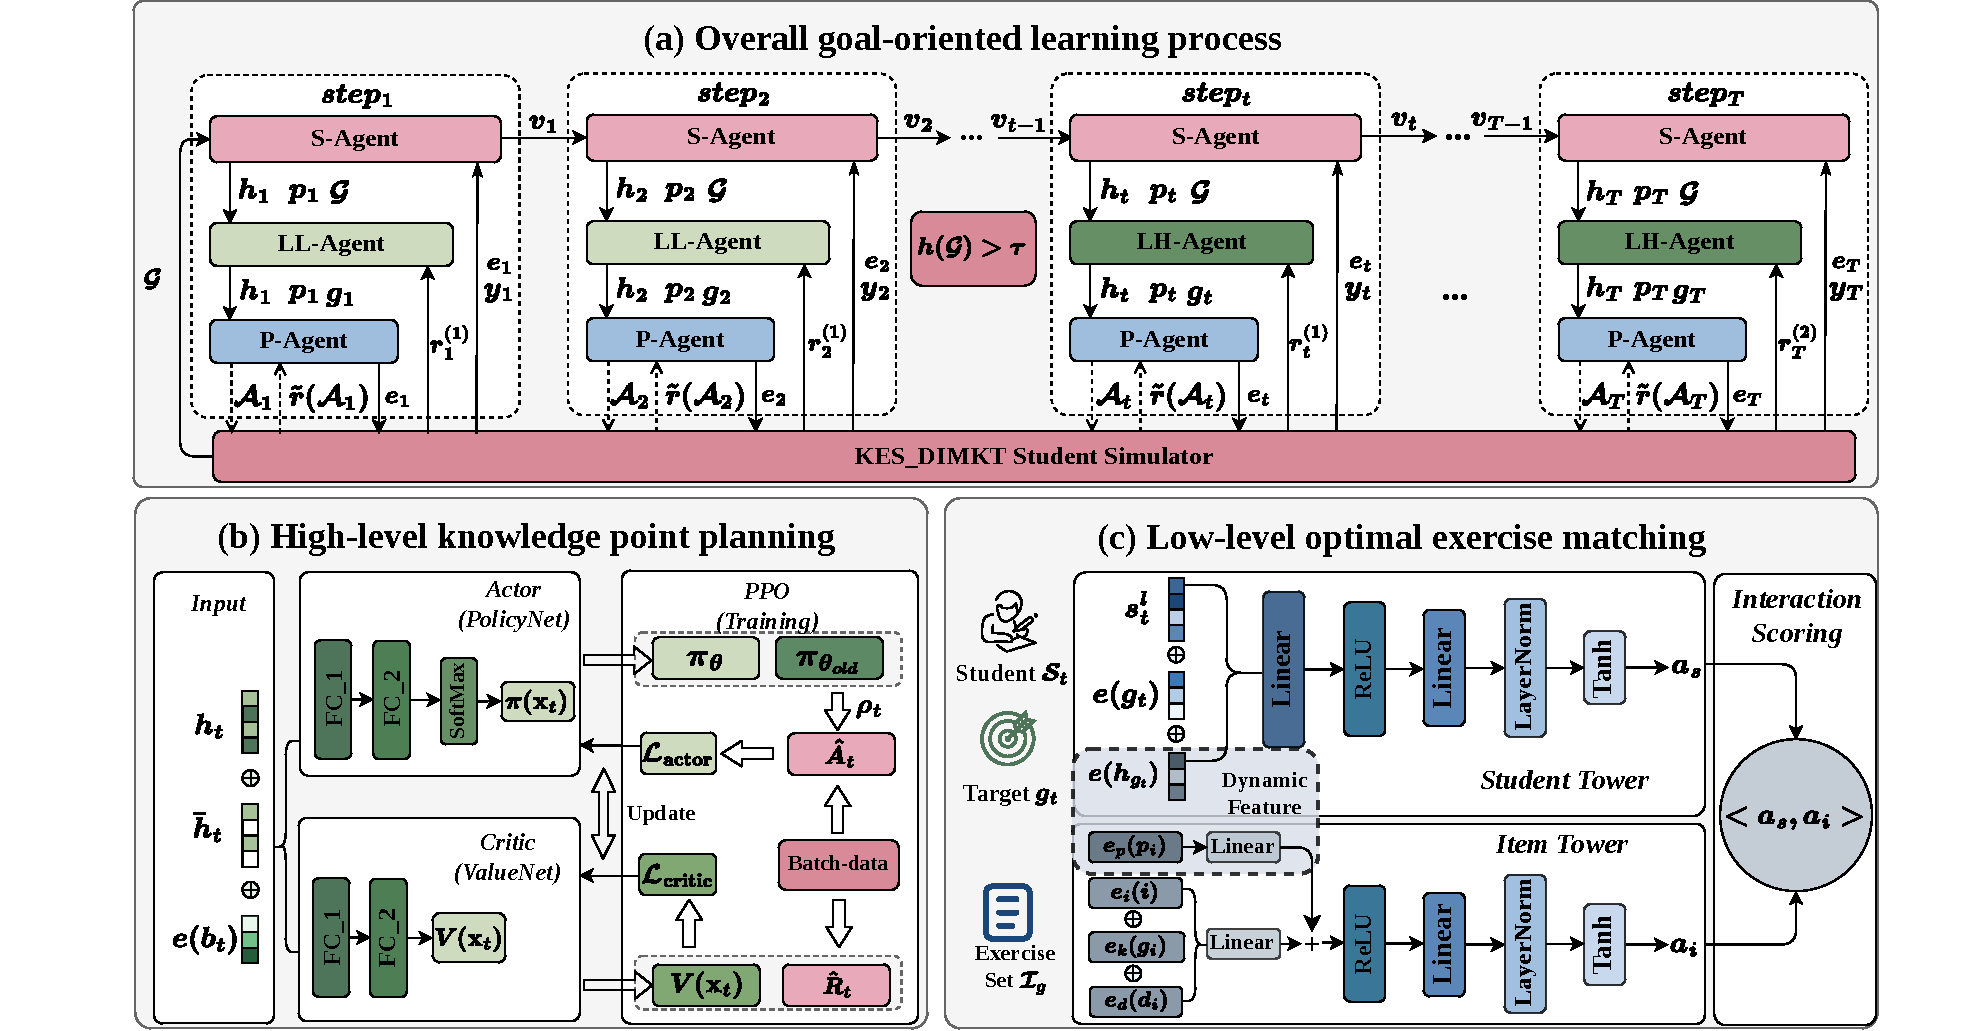
\includegraphics[width=1.0\textwidth]{framework.pdf} % 换成你的图
  \caption{\textbf{Framework overview of FGLP.} (a) The overall goal-oriented learning process alternates between state estimation, high-level knowledge point planning, low-level exercise selection, and simulator feedback. (b) The high-level layer performs two-stage knowledge point planning for target promotion and target consolidation. (c) The low-level layer uses a state-aware two-tower matching model to select the exercise that best serves the current knowledge point.}
  \label{fig:framework}
\end{figure*}
如图~\ref{fig:framework} 所示，本文框架由学生状态估计模块 S-Agent、知识点推荐层、习题推荐层以及底部学生模拟器共同组成，并按照“状态估计 $\rightarrow$ 知识点决策 $\rightarrow$ 习题决策 $\rightarrow$ 交互反馈”的流程形成逐步闭环，其形式化定义已在 Problem Formulation 中给出。图~\ref{fig:framework}(a) 展示了整体目标导向学习过程：在每个决策步，系统首先根据历史交互估计学生当前的知识点状态与题目状态，再由高层确定当前应服务的学习知识点，随后由低层围绕该知识点完成局部习题选择，最终通过学生模拟器返回新的反馈状态，用于驱动下一步决策。

图~\ref{fig:framework}(b) 对应知识点推荐层。该层负责路径的全局推进，回答“下一步最值得学习哪个知识点”。与传统单策略高层不同，本文在知识点层L-Agent显式引入双阶段机制：当目标知识点尚未达到掌握阈值时，LL-Agent的策略是优先推动目标完成；当目标已经达成且预算仍有剩余时，系统切换到LH-Agent，维持并巩固已达成的目标状态。图~\ref{fig:framework}(c) 对应习题推荐层P-Agent。该层负责局部实例化，回答“围绕当前知识点最适合练习哪一道题”。在当前学习知识点约束下，习题层先通过两塔匹配建模学生与候选题之间的适配关系，再结合一步前瞻收益构造监督信号，从而学习面向局部学习增益的选题函数。

需要强调的是，图~\ref{fig:framework}(a)中的 S-Agent 与底部学生模拟器虽然都建立在预训练DIMKT模型之上,但它们并不共享同一组参数，而是分别对应两套相近但不等同的预训练模型。具体而言，S-Agent 服务于决策侧状态估计，而学生模拟器服务于环境侧状态演化。这一点与真实在线教育场景更为一致，因为推荐系统通常只能基于历史交互去推断学生掌握状态，而不可能无偏、无噪声地直接获得真实知识状态。

\subsection{知识点推荐层}
知识点推荐层承担全局规划的职责，其目标是在当前学生状态与剩余预算约束下，确定下一步最值得学习的知识点，以提升目标知识点集合 $\mathcal{G}_{target}$ 的整体掌握程度。

\subsubsection{状态建模}

结合图~\ref{fig:framework}(b) L-Agent 结构，我们将真正输入神经网络的状态信息压缩为三部分：学生当前的知识点掌握状态 $h_t$、目标感知状态 $\bar{h}_t=h_t\odot y$ 以及预算嵌入 $e_b(b_t)$。其中，$y\in\{0,1\}^{|\mathcal{K}|}$ 为目标指示向量，当 $k\in\mathcal{G}_{target}$ 时有 $y(k)=1$，否则为 $0$；因此，$\bar{h}_t$ 用于突出目标集合上的实时学习进展。基于上述表示，我们将高层状态定义为
\begin{equation}
s_t^h=[h_t;\,\bar{h}_t;\,e_b(b_t)],
\end{equation}
这样设计的动机在于：$h_t$ 提供学生的全局知识背景，$\bar{h}_t$ 则显式刻画与目标集合 $\mathcal{G}_{target}$ 直接相关的掌握状态，而 $e_b(b_t)$ 进一步反映“还剩多少决策空间”。


\subsubsection{双阶段目标导向与策略生成}

真实学习过程通常包含两个相互衔接但目标不同的阶段：首先需要尽快推动目标知识点达到掌握阈值，其次还需要在预算允许的情况下维持并强化已经达成的目标状态。若仅使用单一策略统一处理这两类决策，容易出现两种偏差：一是在目标尚未完成时过早转向巩固，降低目标推进效率；二是在目标刚刚达到阈值后立即转向其他知识点，导致目标状态不稳定。因此，我们在知识点层采用双阶段目标导向决策机制。

具体而言，我们首先根据目标集合在当前时刻的掌握情况判定所处阶段。当仍存在未达到掌握阈值 $\tau$ 的目标知识点时，系统激活LL-Agent；当全部目标知识点均达到阈值且预算仍有剩余时，系统自动切换到LH-Agent。

在策略生成阶段，我们使用策略网络根据当前高层状态 $s_t^h$ 生成对所有知识点的条件分布，并从中选出当前应当学习的知识点 $g_t$。我们将阶段 $m\in\{1,2\}$ 的策略网络和价值网络均实现为前馈全连接网络，其形式分别写为
\begin{equation}
\begin{aligned}
\pi_{\theta_m}^h( s_t^h)
&=
\mathrm{Softmax}\!\big(FC_{\theta_m}(s_t^h)\big),\\
\qquad
V_{\phi_m}(s_t^h)&=FC_{\phi_m}(s_t^h).
\end{aligned}
\end{equation}
其中，$FC_{\theta_m}(\cdot)$ 和 $FC_{\phi_m}(\cdot)$ 分别表示策略侧与价值侧的前馈神经网络。策略网络输出当前状态下各知识点的选择分布，价值网络则估计该状态对应的长期回报。

\subsubsection{奖励设计}

为了使双阶段策略与其优化目标保持一致，我们分别为两个不同阶段的L-Agent设计不同的奖励函数。在阶段一，记时刻 $t$ 的二元学习收益与连续学习收益分别为 $E_t^{N}$ 和 $E_t^{S}$。于是，阶段一的一步奖励可写为
\begin{equation}
r_t^{h,1}
=
\Delta E_t^{N}
+
\Delta E_t^{S}
-
\eta
-
\xi_t,
\end{equation}
其中 $\Delta E_t^{N}=E_{t+1}^{N}-E_t^{N}$，$\Delta E_t^{S}=E_{t+1}^{S}-E_t^{S}$，$\eta$ 为一个固定值得步级惩罚项，而 $\xi_t$ 表示预算约束下的终局惩罚，其惩罚幅度记为 $\xi=\lambda_{\xi}(1-E_T^{N})$。该奖励同时刻画两类学习收益：一类是目标知识点跨越掌握阈值所带来的离散完成增益，另一类是目标集合整体掌握水平上升带来的连续收益增益。前者鼓励策略优先完成尚未达标的目标知识点，后者则避免策略仅追求二值化的“是否达标”，而忽略目标集合内部更细粒度的学习进展。当预算耗尽而目标仍未完成时，引入终局惩罚能够抑制无效探索，使阶段一策略更加聚焦于有限预算下的目标推进。步级惩罚项与状态建模中的预算嵌入共同服务于同一目标，即在有限预算约束下提高知识点规划效率。通过这种状态侧与奖励侧的一致性设计，我们能够使 L-Agent 在生成决策时具备预算感知能力，并在学习过程中进一步强化对预算使用效率的偏好。

当全部目标知识点均达到阈值且预算仍有剩余时，系统进入阶段二。此时，LH-Agent不再将“达标”作为主要优化方向，而是转而强调目标状态的稳定保持与进一步提升。阶段二奖励定义为:
\begin{equation}
r_t^{h,2}=2\Delta E_t^{S}-
\mu\,\mathbb{I}\!\left(\exists k\in\mathcal{G}_{target},\,h_{t+1}(k)<\tau\right)
-
\eta,
\end{equation}
其中 $\mu$ 为退化惩罚系数。与阶段一相比，阶段二不再关注“有多少目标基本合格”，而是更关注“已完成目标能否继续提高”。一旦某个目标知识点在后续交互中重新跌破阈值，系统便施加退化惩罚，从而抑制策略在巩固阶段偏向无关知识点或高风险知识点。

\subsubsection{策略学习}

我们采用 PPO 对知识点策略进行优化.给定一条由知识点决策形成的交互轨迹，首先根据时序差分误差构造优势项：
\begin{equation}
\begin{aligned}
\delta_t &= r_t^{h,m}+\gamma V_{\phi_m}(s_{t+1}^h)-V_{\phi_m}(s_t^h),\\
\hat{A}_t &= \sum_{l=0}^{\infty}(\gamma\lambda)^l\delta_{t+l}.
\end{aligned}
\end{equation}
其中，$\gamma$表示折扣因子,$\lambda\in[0,1]$ 为 广义优势估计(GAE)中的衰减系数，用于调节优势估计在偏差与方差之间的权衡；较大的 $\lambda$ 使估计更多吸收长时域回报信息，而较小的 $\lambda$ 则使其更接近局部时序差分更新。随后，策略网络通过 PPO 裁剪目标进行更新：
\begin{equation}
\mathcal{L}_{actor}^{(m)}
=
-\mathbb{E}_t
\left[
\min\left(
\rho_t\hat{A}_t,\,
\mathrm{clip}(\rho_t,1-\epsilon,1+\epsilon)\hat{A}_t
\right)
\right],
\end{equation}
其中 $\rho_t=\pi_{\theta_m}^h(g_t\mid s_t^h)/\pi_{\theta_m^{old}}^h(g_t\mid s_t^h)$。为了与策略侧更新相对应，价值网络并非直接回归原始累积奖励，而是先基于冻结的价值估计构造 TD($\lambda$) 式目标回报，再用当前价值网络进行拟合，即
\begin{equation}
\hat{R}_t^{(m)}=\hat{A}_t+\hat{V}_{\phi_m}(s_t^h),
\end{equation}
并通过最小化平方误差来更新参数：
\begin{equation}
\mathcal{L}_{critic}^{(m)}
=
\mathbb{E}_t\left[
\left(
V_{\phi_m}(s_t^h)-\hat{R}_t^{(m)}
\right)^2
\right].
\end{equation}
其中 $\hat{V}_{\phi_m}(s_t^h)$ 表示在当前更新轮次开始时计算得到的价值基线。这样的设计使得价值函数学习与优势估计保持一致，并避免在构造回归目标与执行参数更新时使用同一个可变预测量，从而为策略更新提供更稳定的基线。由于我们为两个阶段分别维护独立的 L-Agent，因此阶段一与阶段二的轨迹也分别用于对应策略的更新。每个阶段都可以围绕自身的优化目标形成更稳定的价值估计和更清晰的策略偏好。
\subsection{习题推荐层}
在高层给定当前学习知识点 $g_t$ 后，我们为了回答“围绕应练习哪一道题目最能够提升学习知识点的掌握水平”,采用图~\ref{fig:framework}(c)所示的两塔结构学习“学生-习题”匹配函数,并将其建模为一个监督式的学习过程.

\subsubsection{双塔匹配建模}

学生塔用于在当前学习知识点条件下生成学生侧状态表示。其输入由三部分组成：学生基础表征 $s_t^l=[p_t;\,h_t]$，其中 $p_t$ 和 $h_t$ 分别表示题目级与知识点级掌握状态；当前学习知识点的语义条件 $e_k(g_t)$；以及学生对该知识点的动态掌握特征 $e_h(h_t(g_t))$，用于突出当前局部学习需求。三类信息共同输入学生侧编码器，得到:
\begin{equation}
a_t^{u}
=
f_u\!\left([s_t^l;\,e_k(g_t);\,
e_h(h_{g_t})]\right),
\end{equation}
其中，$f_u(\cdot)$ 对应于图~\ref{fig:framework}(c)中的学生塔前馈编码网络。$a_t^u$ 表示知识点条件化的学生侧表示。相应地，前文所述的局部决策上下文 $c_t^l$ 可以理解为由学生基础状态、当前知识点语义条件及其动态掌握特征共同构成的上下文输入。

与之对应，习题塔同时整合习题静态特征与学生-习题交互相关的动态特征。对于任意候选习题 $i$，我们将题目标识嵌入$e_i(i)$、所属知识点嵌入$e_k(k_i)$与题目难度嵌入$e_d(d_i)$视为其静态描述.在此基础上，再引入题目级掌握度嵌入 $e_p(p_t(i))$ 作为动态补充，并通过线性变换将其与静态表示融合，进而得到习题表示:
\begin{equation}
a_i^{v}
=
f_v\!\left(
W_s[e_i(i);\,
e_k(k(i));\,
e_d(d_i)]
+
W_p e_p(p_i)
\right),
\end{equation}
其中$W_s$ 与 $W_p$ 分别表示静态特征映射与动态特征映射，$f_v(\cdot)$ 为习题侧输出网络,$a_i^v$ 表示动态化的习题侧表示。于是，习题塔的表示学习形成了“静态特征先映射、动态特征再注入”的结构：前者用于描述题目本身，后者用于表征学生当前对该题的熟悉程度。

在此基础上，我们采用内积形式衡量学生表示与习题表示之间的匹配强度，并将其作为当前状态下的习题适配得分输出：
\begin{equation}
\hat{r}_{t}(i\mid c_t^l,g_t)=\langle a_t^{u},a_i^{v}\rangle.
\end{equation}
该得分并不直接等价于作答正确概率，而是刻画题目 $i$ 在当前学习知识点 $g_t$ 及当前学生状态下的练习适配性。分数越高，表示该题越可能在当前局部学习阶段发挥有效练习作用。
\subsubsection{候选生成}

围绕当前学习知识点 $g_t$ 的习题选择，并不是直接在全题库上进行，而是先构造一个与当前学习阶段相匹配的合法候选集合 $\mathcal{I}_g$。在实现上，我们首先依据知识点到习题的映射关系 $\mathcal{M}(k)$ 收集与知识点 $k$ 相关的题目集合。同时,我们并不将候选范围限制为 $\mathcal{M}(g_t)$，而是进一步结合知识结构图为 $g_t$ 引入一对邻近知识点：记
\begin{equation}
\begin{aligned}
\tilde{k}_t^{-}
&=
\arg\min_{k\in \mathrm{Pre}(g_t)} h_t(k),\\\qquad
\tilde{k}_t^{+}
&=
\arg\max_{k\in \mathrm{Suc}(g_t)} h_t(k),  
\end{aligned}
\end{equation}
其中 $\mathrm{Pre}(g_t)$ 与 $\mathrm{Suc}(g_t)$ 分别表示 $g_t$ 在知识图中的前置知识点集合与后继知识点集合。前者用于定位当前最薄弱的先修支撑点，后者用于定位当前掌握程度较高的后继关联点。于是，合法候选集合定义为
\begin{equation}
\mathcal{I}_t(g_t)
=
\mathcal{M}(g_t)\cup
\mathcal{M}(\tilde{k}_t^{-})\cup
\mathcal{M}(\tilde{k}_t^{+})
,
\end{equation}
当某一邻域集合为空时，对应项自然省略。上述设计使候选题既覆盖当前学习知识点本身，也保留一小部分与其直接相关的先修和后继题目，从而为局部选题保留必要的结构弹性。在得到合法候选集合后，我们再由两塔网络在该集合上输出习题适配得分，并形成一个用于后续训练决策的小规模候选子集
\begin{equation}
\mathcal{A}_t
=
\mathrm{TopK}\!\left(\hat{r}_{t}(\cdot\mid c_t^l,g_t),K\right)
\cup
\mathrm{Rand}\!\left(\mathcal{I}_t(g_t),K_r\right).
\end{equation}
其中，$K$ 表示由两塔匹配得分筛出的高分候选数，$K_r$ 表示为保持候选多样性而额外加入的随机候选数。

\subsubsection{题目选择与监督学习}

在训练阶段，P-Agent 并不直接把两塔打分最高的题目作为最终执行题目，而是对候选题进行一步前瞻评估。具体地，对于每个候选习题 $i\in\mathcal{A}_t$，记其对应的一步前瞻知识状态为 $\hat{h}_{t+1}^{(i)}$，并令
\begin{equation}
\tilde{r}_t(i)=
\hat{h}_{t+1}^{(i)}(g_t)-h_t(g_t),
\end{equation}
该收益一方面决定训练阶段真实执行的题目 $e_t$，另一方面也为同组候选样本提供监督信号，使 P-Agent 学习当前状态下更可靠的局部选题规则。

在监督学习时，我们会保留同一候选集合 $\mathcal{A}_t$ 中题目的 $(c_t^l,g_t,e_t,\tilde{r}_t(e_t))$。这样，模型能够同时观察“最终被选中的题目”与“在同一状态下未被选中的备选题目”，从而学习更稳定的局部偏序关系。记 $\bar{r}_t(i)$ 为对 $\tilde{r}_t(i)$ 进行组内标准化后得到的监督信号，则习题推荐层的训练目标写为
\begin{equation}
\begin{aligned}
\mathcal{L}_{grp}
&=
\frac{1}{|\mathcal{P}_t|}
\sum_{(i,j)\in\mathcal{P}_t}
\mathrm{softplus}\!\big(
\hat{r}_{t}(j)-\hat{r}_{t}(i)
\big),\\
\mathcal{L}_{reg}
&=
\mathrm{SmoothL1}\!\left(
\hat{r}_{t}(i\mid c_t^l,g_t),\bar{r}_t(i)
\right),\\
\mathcal{L}_{P}
&=
\lambda_{grp} \mathcal{L}_{grp}
+
\lambda_{reg} \mathcal{L}_{reg},
\end{aligned}
\end{equation}
其中，$\mathcal{P}_t=\{(i,j)\mid \tilde{r}_t(i)>\tilde{r}_t(j)\}$ 表示由模拟收益诱导的候选偏序集合；$\lambda_{grp}$ 与 $\lambda_{reg}$ 分别控制组内排序约束与收益回归约束的强度。前者推动模型在同一候选组内学习“哪道题更优”，后者则使预测得分与收益监督保持数值一致。由此，训练阶段的 P-Agent 本质上是在当前学习知识点 $g_t$ 条件下，借助一步前瞻收益构造监督信号，并学习一个能够识别最合适练习题的局部匹配函数。

在推理阶段，我们不再使用上述一步前瞻收益来重排候选题目，而是直接依据P-Agent已经学得的两塔匹配在合法候选集内完成选题。
\begin{table}[H]
\centering
\captionsetup{labelfont=bf,textfont=bf}
\caption{Statistics of the datasets.}
\label{tab:datasets}
\setlength{\tabcolsep}{4pt}
\footnotesize
\begin{tabular}{cccc}
\toprule
\textbf{Dataset} & \textbf{Junyi} & \textbf{Assist09} & \textbf{Assist17}  \\
\midrule
Concept & 39 & 123 & 102 \\
Item & 721 & 17737 & 3162 \\
Learner & 191874 & 3852 & 1708 \\
Interaction & 25,853,987 & 337,424 & 942,814 \\
Difficulty & 26.87 & 34.29 & 53.91 \\
\bottomrule
\end{tabular}
\end{table}
\section{实验}
在这个部分,我们首先介绍我们的实验设置.然后通过丰富的实验证明我们方法的优越性.
\subsection{Datasets}
我们的方法建立在3个公开数据集之上:Junyi,Assist09,Assist17的基础之上.和DLPR一样,我们使用了转移图构建了Assist09和Assist17的知识图谱;根据Junyi数据集提供的一个习题级的先决关系图构建了知识点级的知识图谱;以及使用相同的方案计算知识点和习题的难度.需要提到的是,我们借助pyKT的数据预处理方案对这三个数据集进行处理,按照16:4:5将其划分为训练集,验证集,测试集.表~\ref{tab:datasets}展示了所有数据集的统计详情.

\begin{table*}[t]
\centering
\captionsetup{labelfont=bf,textfont=bf}
\caption{Performance comparison on Junyi, Assist09, and Assist17. The best and second-best results in each row are highlighted in bold and underlined, respectively.}
\label{tab:main_results}
\setlength{\tabcolsep}{3.2pt}
\renewcommand{\arraystretch}{1.0}
\scriptsize
\resizebox{\textwidth}{!}{
\begin{tabular}{cccccccccccc}
\toprule
\textbf{Dataset} & \textbf{Indicator} & \textbf{Step} & \textbf{AC} & \textbf{PPO} & \textbf{GRU4Rec} & \textbf{SRC} & \textbf{CSEAL} & \textbf{GEHRL} & \textbf{DLPR} & \textbf{UNO} & \textbf{FGLP} \\
\midrule
\multirow[c]{6}{*}{Junyi} & \multirow[c]{3}{*}{En} & 5  & 0.2487 & 0.3574 & 0.0912 & 0.4647 & 0.2516 & 0.2038 & \underline{0.5364} & 0.2898 & \textbf{0.5873} \\
 &  & 10 & 0.3407 & 0.5199 & 0.1646 & \underline{0.6410} & 0.3440 & 0.3090 & 0.6350 & 0.4216 & \textbf{0.8326} \\
 &  & 20 & 0.5145 & 0.6697 & 0.2392 & \underline{0.9473} & 0.4327 & 0.4463 & 0.6976 & 0.5666 & \textbf{0.9692} \\
\cmidrule(lr){2-12}
 & \multirow[c]{3}{*}{Es} & 5  & 0.0721 & 0.1286 & 0.0612 & 0.2168 & 0.0514 & 0.0669 & \underline{0.2348} & 0.1181 & \textbf{0.2586} \\
 &  & 10 & 0.1161 & 0.2146 & 0.1749 & \underline{0.3159} & 0.0867 & 0.1042 & 0.2493 & 0.1840 & \textbf{0.4464} \\
 &  & 20 & 0.1836 & 0.3295 & 0.1241 & \underline{0.6205} & 0.1364 & 0.1614 & 0.2746 & 0.2689 & \textbf{0.6761} \\
\midrule
\multirow[c]{6}{*}{Assist09} & \multirow[c]{3}{*}{En} & 5  & 0.3428 & 0.3375 & 0.3293 & 0.3476 & 0.2516 & 0.2867 & 0.1802 & \underline{0.4602} & \textbf{0.6881} \\
 &  & 10 & 0.4079 & 0.4729 & 0.1533 & 0.4205 & 0.3440 & 0.3685 & 0.2175 & \underline{0.4917} & \textbf{0.7496} \\
 &  & 20 & 0.4207 & 0.6063 & 0.1241 & \underline{0.6883} & 0.4143 & 0.4287 & 0.2466 & 0.4947 & \textbf{0.9165} \\
\cmidrule(lr){2-12}
 & \multirow[c]{3}{*}{Es} & 5  & 0.1530 & 0.1892 & 0.1721 & 0.2042 & 0.1128 & 0.1515 & 0.0194 & \underline{0.2269} & \textbf{0.5296} \\
 &  & 10 & 0.1435 & 0.2426 & 0.0058 & \underline{0.2848} & 0.1152 & 0.1476 & -0.0057 & 0.1909 & \textbf{0.5851} \\
 &  & 20 & 0.1382 & 0.3276 & 0.0131 & \underline{0.4318} & 0.1140 & 0.1523 & -0.0197 & 0.1659 & \textbf{0.7397} \\
\midrule
\multirow[c]{6}{*}{Assist17} & \multirow[c]{3}{*}{En} & 5  & 0.2941 & \underline{0.3108} & -0.0468 & 0.1995 & 0.0837 & 0.0191 & 0.1059 & \textbf{0.3796} & 0.2886 \\
 &  & 10 & 0.3747 & 0.4147 & -0.0041 & 0.4047 & 0.1681 & 0.0302 & 0.1920 & \underline{0.4225} & \textbf{0.4711} \\
 &  & 20 & 0.4440 & 0.7071 & 0.0068 & \underline{0.7859} & 0.2967 & 0.0442 & 0.1387 & 0.4386 & \textbf{0.9169} \\
\cmidrule(lr){2-12}
 & \multirow[c]{3}{*}{Es} & 5  & \underline{0.2349} & 0.1861 & 0.0290 & 0.2110 & 0.0953 & 0.0313 & 0.0466 & \textbf{0.2845} & 0.1976 \\
 &  & 10 & 0.2803 & 0.2601 & 0.0655 & 0.2561 & 0.1255 & 0.0289 & 0.0800 & \underline{0.2859} & \textbf{0.3114} \\
 &  & 20 & 0.2665 & 0.3202 & 0.0947 & \underline{0.4350} & 0.1726 & 0.0329 & 0.1039 & 0.2871 & \textbf{0.5765} \\
\bottomrule
\end{tabular}
}
\end{table*}

\subsection{Compared Methods}

为了证明我们方法的优越性,我们与以下方法进行对比:
\begin{itemize}
\item AC:使用DIMKT对学生状态进行建模,在其基础上使用基于步级奖励方式训练的标准Actor-Critic算法作为推荐器\cite{sutton1999policy}.
\item PPO:使用DIMKT对学生状态进行建模,在其基础上使用基于步级奖励方式训练的PPO算法作为推荐器\cite{schulman2017proximal}.
\item GRU4Rec:GRU4Rec 是一种基于 GRU 的序列推荐模型，把用户历史交互看成时间序列，用循环神经网络去预测“下一个最可能交互的项目”\cite{hidasi2015session}。
\item SRC:SRC 是一种 set-to-sequence 的学习路径推荐方法：先把目标知识点集合输入到概念感知编码器中，建模知识点之间的关系并得到整体表示,然后再由解码器根据这个表示按顺序逐步生成学习路径\cite{chen2023set}.
\item CSEAL:CSEAL根据学习者状态并通过使用一种认知导航算法限制强化学习动作空间来指导Actor-Critic网络实现学习路径推荐\cite{liu2019exploiting}.
\item GEHRL:GEHRL使用分层强化学习方法,通过高层 PPO 代理规划多目标学习顺序、低层 Actor-Critic 代理实现单目标的学习\cite{li2023graph}.
\item DLPR:DLPR在分层强化学习的基础上,引入习题层面的考虑,将高层建模为基于PPO和A*算法的知识点学习规划,将低层建模为基于Actor-Critic的具体知识点的练习规划\cite{zhang2024item}.
\item UNO:UNO是一种基于序列编码的强化学习推荐方法，它首先对学生历史作答序列进行表示学习以构建当前状态，再结合知识追踪辅助监督与 GRPO 式策略优化实现下一习题推荐\cite{peng2026uno}。
\end{itemize}

\subsection{Implementation Detail}
我们基于 PyTorch\cite{paszke2019pytorch}、Gym\cite{brockman2016openai}实现整个框架，并采用 pyKT提供的代码对 DIMKT 进行预训练。将基于训练集训练得到的 DIMKT 模型作为S-Agent的核心，以提供决策侧的学生状态估计；将基于训练集与测试集合并数据训练得到的另一套 DIMKT 模型作为学生的模拟器，以刻画环境侧更接近真实演化过程的状态转移。

在当前实现中，知识点层采用两个独立的 PPO 智能体分别对应目标推进阶段与目标巩固阶段。参考在线教育中常用的及格标准，我们将知识点掌握阈值设置为 0.6，并将单个学习会话的最大决策预算限制为 20 步。与前文奖励设计对应，步级惩罚系数和终局惩罚系数分别取 0.03 和 1.0。习题层采用双塔 Bandit 实现局部监督式选题，在候选重排阶段，系统从合法候选集合中保留 6 道高分题，并额外补充 10 道随机候选题，以兼顾候选质量与局部探索。训练阶段，P-Agent 使用一步前瞻收益对候选题进行监督，并联合优化组内排序损失与回归损失；两类损失的权重分别设置为 0.1 和 1.0。对于知识点层PPO代理，我们使用 Adam\cite{kingma2014adam} 来优化 Actor 和 Critic 网络，这符合在策略内策略梯度训练中的常见做法。对于低层双塔习题选择器，我们采用带有小权重衰减的 AdamW\cite{loshchilov2017decoupled} 来规范化监督匹配模型，并减少对本地候选练习的过拟合。

\subsection{Experiment Result}
表~\ref{tab:main_results}显示了本文方法在三个数据集上的大多数设置下都取得了最优结果，说明所提出的分层两阶段细粒度决策框架能够稳定提升目标导向学习路径推荐的整体效果。尤其在 Junyi 和 Assist09 上，本文方法在不同步数与两类指标下均表现出显著优势；在 Assist17 上，仅在 $Step=5$ 的极短学习过程中略低于个别基线。我们认为，这并非短期失效，而是面向长期目标优化的阶段性取舍：为在有限预算内最大化最终学习收益，本文方法在前 5 步更倾向于为后续阶段积累更有利的知识状态，因此虽在
\begin{figure}[t] % 位置参数，见下文解释
    \centering % 图片居中
    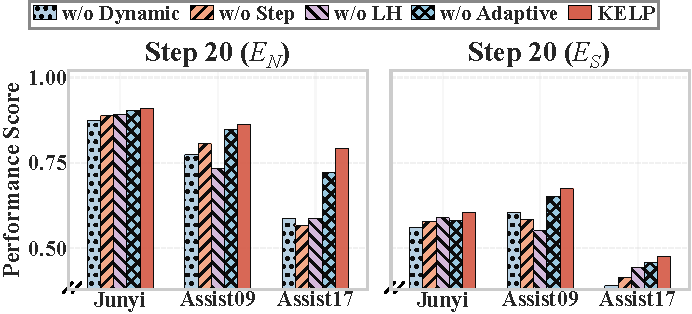
\includegraphics[width=0.9\columnwidth]{ablation_study_step20.pdf} % 插入图片并设置宽度
    \caption{Ablation study of each optimization module}
    \label{fig:Ablation study} % 用于交叉引用的标签
\end{figure}短期上略有让步，但在 $Step=10$ 与 $Step=20$ 时重新取得最优结果。

进一步观察基线方法可以发现，AC 与 PPO 虽然建模更简单，但在多数设置下整体优于 CSEAL 和 GEHRL，并在部分场景下接近甚至超过 UNO。这表明，合理的奖励机制对学习路径推荐性能具有关键作用：即使不引入复杂结构，只要奖励能够准确反映学习增益，系统依然能够学到较优策略。SRC 同样表现出较强竞争力，其重要原因在于编码器--解码器框架支持大批量并行训练，能够在更短时间内利用更多学生数据，具有明显的工程化优势；相比之下，其余强化学习方法大多依赖串行交互训练。即便如此，本文方法仍在绝大多数设置下超越 SRC，说明将连续学习收益、双阶段知识点决策与面向局部增益的习题选择统一起来，能够进一步提升目标导向学习路径推荐的性能上限。

\begin{figure*}[t] % 位置参数，见下文解释
    \centering % 图片居中
    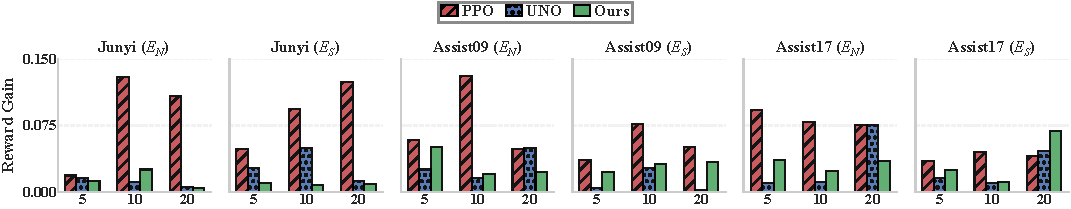
\includegraphics[width=0.98\textwidth]{p1_p12_diff_comparison.pdf} % 插入图片并设置宽度
    \caption{Reward transfer study. The vertical axis denotes the average performance gain, computed as $\text{Composite Reward}-\text{Binary-Only Reward}$.}
    \label{fig:diff-comparison} % 用于交叉引用的标签
\end{figure*}
\subsection{Ablation Study}
在图~\ref{fig:Ablation study}中,为分析关键模块的作用，我们在主模型基础上设计四个消融变体：w/o Dynamic 去除习题层动态特征，w/o step 去除剩余步数特征及对应步级惩罚，w/o L2 移除阶段二知识点策略，w/o Adaptive 移除自适应候选机制。从结果上看，完整模型在大多数设置下均取得最优表现，说明上述设计均对性能提升有积极作用。其中，去除动态特征后性能明显下降，表明状态感知的局部匹配对习题推荐至关重要；去除预算感知后，中长预算下表现普遍变差，说明剩余步数特征及步级惩罚有助于提升知识点层的规划效率；移除阶段二策略后，部分连续收益指标 $E_S$ 下降更明显，说明独立的巩固阶段策略能够提升后期目标保持与强化效果；移除自适应候选机制后，模型在多个数据集上均出现退化，说明基于当前知识点及其邻域动态构造候选集合能够提升局部选题质量。

\subsection{Reward Transfer Study}
为验证知识点层细粒度奖励设计的可迁移性，我们在 PPO、UNO 和本文方法上比较两种步级奖励设置：仅使用二元收益增量 $\Delta E_t^{N}$ 的 \textbf{Binary-Only Reward}，以及同时使用 $\Delta E_t^{N}+\Delta E_t^{S}$ 的 \textbf{Composite Reward}。其中，$\Delta E_t^{S}$ 与前文 L-Agent 奖励函数中的连续收益项一致，用于提供更细粒度的知识状态变化信号。图~\ref{fig:diff-comparison}展示的是两种设置下平均学习收益的差值，即 $\text{Composite Reward} - \text{Binary-Only Reward}$。可以看到，大多数结果均大于 0，说明在不同方法和不同数据集上，引入 $\Delta E_t^{S}$ 后整体都能带来稳定增益。进一步观察可以发现，PPO 的增益效果最为明显，说明合理的奖励机制对普通强化学习模型的影响更大；当模型结构相对简单时，细粒度奖励信号能够更直接地引导策略优化。这表明连续收益项不仅对本文方法有效，也具有较好的方法无关性与可迁移性。
\begin{table}[t]
\centering
\captionsetup{labelfont=bf,textfont=bf}
\caption{\textbf{Stability comparison under different L-Agent algorithms.}}
\label{tab:stability_analysis}
\setlength{\tabcolsep}{2.6pt}
\renewcommand{\arraystretch}{1.0}
\scriptsize
\begin{tabular}{ccccccc}
\toprule
\textbf{Dataset} & \textbf{Indicator} & \textbf{Step} & \textbf{AC} & \textbf{DQN} & \textbf{SAC} & \textbf{PPO} \\
\midrule
\multirow[c]{6}{*}{as09} & \multirow[c]{3}{*}{En} & 5  & 0.4933 & 0.3765 & 0.4706 & \textbf{0.6881} \\
 &  & 10 & 0.5427 & 0.3802 & 0.4593 & \textbf{0.7496} \\
 &  & 20 & 0.6221 & 0.5521 & 0.6487 & \textbf{0.9165} \\
\cmidrule(lr){2-7}
 & \multirow[c]{3}{*}{Es} & 5  & 0.3442 & 0.2691 & 0.3501 & \textbf{0.5296} \\
 &  & 10 & 0.3876 & 0.2513 & 0.3702 & \textbf{0.5851} \\
 &  & 20 & 0.4543 & 0.3948 & 0.4786 & \textbf{0.7397} \\
\midrule
\multirow[c]{6}{*}{as17} & \multirow[c]{3}{*}{En} & 5  & 0.2346 & 0.2241 & 0.2456 & \textbf{0.2886} \\
 &  & 10 & 0.3986 & 0.4156 & 0.4205 & \textbf{0.4711} \\
 &  & 20 & 0.6567 & 0.6319 & 0.6778 & \textbf{0.9169} \\
\cmidrule(lr){2-7}
 & \multirow[c]{3}{*}{Es} & 5  & 0.1763 & 0.1698 & 0.1816 & \textbf{0.1976} \\
 &  & 10 & 0.2642 & 0.2482 & 0.2523 & \textbf{0.3114} \\
 &  & 20 & 0.3968 & 0.3833 & 0.4482 & \textbf{0.5765} \\
\bottomrule
\end{tabular}
\end{table}
\subsection{Stability Analysis}

为验证整体框架在更换知识点层算法后的稳定性，我们固定习题推荐层不变，仅将 L-Agent 分别替换为 AC、DQN\cite{mnih2015human}、SAC\cite{haarnoja2018soft} 和本文采用的 PPO 版本，并统计不同步数下的平均学习收益。表~\ref{tab:stability_analysis} 表明，使用 PPO 的本文方案在两个数据集上的 $E_N$ 和 $E_S$ 指标上整体最优；同时，无论采用哪种知识点策略，学习收益都能随步数增加而逐步提升，说明在更换 L-Agent 后，整体双层推荐框架仍能保持较稳定的优化趋势。进一步地，可以看到 DQN 在大多数设置下都落后于 AC、SAC 和 PPO，说明仅依赖价值估计的离散动作策略在当前知识点规划任务上相对较弱，而 actor-critic 类方法能够更好地适应该类序列决策过程。该结果从侧面说明，本文方法不仅在算法选择上具有优势，也具有较好的结构稳定性。


\subsection{P-Agent Effectiveness Analysis}
为进一步验证 P-Agent 评分机制的有效性，我们在测试阶段分别执行排序第 1 至第 5 的候选习题，并比较不同选择下的最终表现，如图~\ref{fig:effctiveness Analysis}。其中，等级 1 表示当前状态下由 P-Agent 判定为$\hat{r}_{t}$分数最高的习题，等级越大表示所选习题在候选集合
中的匹配分数越低。从结果来看，三个数据集整体上都呈现出一致趋势：随着所选习题的等级从 1 下降到 5，$E_N$ 与 $E_S$ 均整体下降，说明 P-Agent 给出的分数能够较好反映习题对当前学习状态的真实适配性。其中，Junyi 与 Assist17 上的下降更为明显，尤其在步数较大时，高排名习题与低排名习题之间的差距进一步拉大；相比之下，Assist09 上不同排序之间的差距相对更平缓，但最优结果仍出现在排序最靠前的位置。总体而言，该实验说明 P-Agent 的评分不仅能够用于候选重排，而且与真实学习收益具有较强一致性，从实验上支持了本文习题推荐层设计的合理性。
\begin{figure}[t] % 位置参数，见下文解释
    \centering % 图片居中
    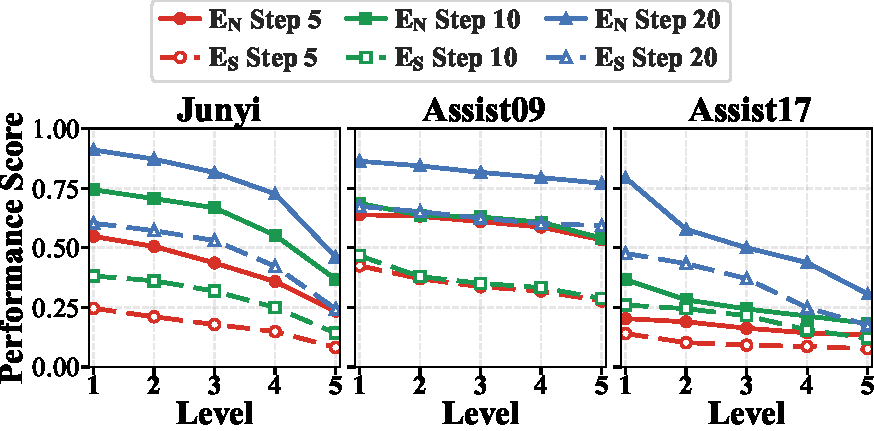
\includegraphics[width=\columnwidth]{adaptability_experiment_font_large.pdf} % 插入图片并设置宽度
    \caption{Comparison of P-Agent performance on exercises of different score levels}
    \label{fig:effctiveness Analysis} % 用于交叉引用的标签 
\end{figure}
\begin{figure}[t]
\centering
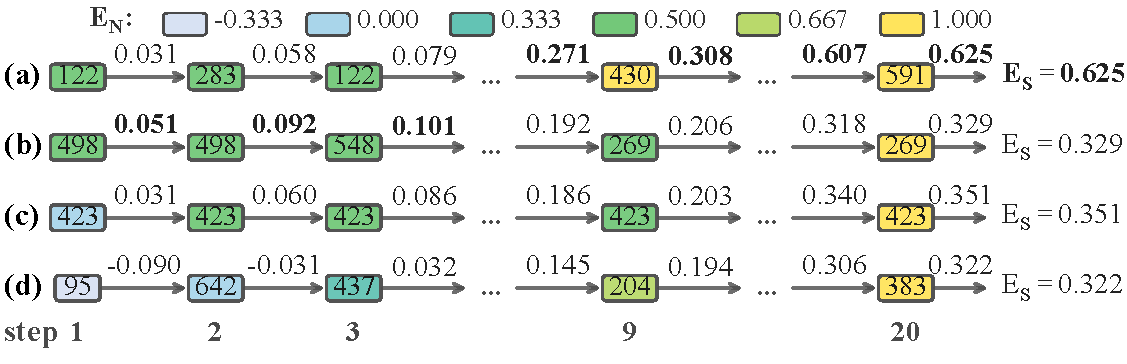
\includegraphics[width=\columnwidth]{case_study.pdf}
\captionsetup{labelfont=bf,textfont=bf}
\caption{Curriculum path case study. (a), (b), (c), and (d) denote FGLP, PPO, UNO, and SRC, respectively.}
\label{fig:case_study}
\end{figure}
\subsection{Case Study}
为进一步分析不同方法的推荐行为，我们展示一个学习路径案例，如图~\ref{fig:case_study} 所示。可以看到,$E_N$指标并不能在每一步都发生变化,当只使用二元收益增量作为过程奖励不可避免地出现为0的情况,从而影响对于这一步动作有效性的判断,这显示地证明了引入连续收益构建细粒度的奖励机制的重要性.我们的方法最快将学习目标推进到合格水平，表现出更高的目标达成效率。进一步地，图中的 (a)、(b) 和 (c) 都属于基于步级过程奖励构建的方法，因此在学习过程中整体收益保持逐步上升，没有出现明显的中途退化；相比之下，使用终局奖励的 SRC 在初始阶段出现了学习收益下降，这种现象在真实学习场景中可能打击学生的学习积极性，并削弱其对推荐系统的信任。另一个值得注意的现象是，UNO 在该案例中多次重复推荐同一道习题，这与数据中存在连续重复练习同一题目的情况有关；由于 UNO 属于序列式推荐方法，更容易捕捉并放大这类模式。但在真实学习过程中，连续多次练习同一道题的情况并不常见，因此推荐系统除了关注收益提升外，也应尽量保持习题推荐的多样性。
\section{Conclusion}
本文针对目标导向学习路径推荐中细粒度状态变化难以刻画、高低层决策反馈不足以及有限预算感知不足的问题，提出了一种基于分层两阶段决策的细粒度学习路径推荐框架 FGLP。该框架通过学生状态估计模块同时建模知识点级与习题级掌握状态，并采用“一步一知识点一习题”的决策粒度，使习题交互后的状态变化能够及时反馈至知识点推荐层。在此基础上，知识点层结合目标推进与目标巩固两阶段策略、连续学习收益和预算感知奖励进行全局规划，习题层则利用状态感知的两塔匹配与 bandit 式局部决策选择更符合当前学习需求的练习题。

在 Junyi、Assist09 和 Assist17 三个公开数据集上的实验结果表明，FGLP 在多数设置下取得了更优的学习收益。消融实验进一步验证了动态特征、预算感知、阶段二策略和自适应候选机制的作用；奖励迁移实验说明连续收益项对不同强化学习方法均具有一定增益，尤其对普通 PPO 模型的影响更为明显；P-Agent 有效性分析和案例研究也表明，本文习题层评分与真实学习收益具有较强一致性。未来工作将进一步结合真实在线学习平台中的交互数据验证框架的实际适用性，并探索更复杂学习目标和长期学习场景下的路径推荐策略。
\printbibliogCEraphy
\end{document}





